\chapter{Parallel Multilevel Multiscale Solver}
\chaptermark{Parallel Multilevel Multiscale Solver}
\label{ch:parallel_multiscale}

The goal of a multiscale solver framework is to accelerate the linear solution of large linear systems arising in high fidelity simulations.   To this end, the solver must exhibit not only algorithmic scalability explored earlier in \cref{ch:multiscale_poromechanics}, but also implementation scalability, i.e. the ability to maintain parallel execution efficiency on large computing clusters.   The ultimate performance measure of a preconditioner is time-to-solution, i.e. a combination of the time it takes to pre-compute and populate data structures for a given linear system (setup time) and the time taken by the iterative scheme to arrive at the solution, which a combination of the number of iterations and the cost per iterations.   To demonstrate scalability, we implemented the methods proposed in \cref{ch:multiscale_poromechanics} in the parallel simulation framework presented in \cref{ch:geosx_framework}, building on the efficient data structures, programming models and interfaces to state-of-the-art linear algebra packages that the framework provides.   This chapter is organized as follows. \Cref{sec:par_implementation} describes the adaptation of the algorithms to parallel environments (both shared and distributed memory) and justifies the design decisions and trade-offs.   In \cref{sec:par_kernels} we analyze in detail the performance of each of the computational kernels that make up the setup and solution phases of the preconditioner.   \Cref{sec:par_results} presents an investigation into parallel efficiency and scalability using several challenging test cases with both structured and unstructured grids, and compares overall performance of the preconditioner to state-of-the-art multigrid methods.    Finally, we conclude with a summary in \cref{sec:par_summary}.

% ===================== SECTION =====================
\section{Parallel Implementation and Data Structures}
\label{sec:par_implementation}

\subsection{General Multilevel Preconditioner Design}
\label{subsec:par_impl_prec_design}

We begin by describing the overall structure of the developed preconditioning framework.   While present work focuses on a specific flavor of multiscale methods, it is important to keep the high-level code design general enough that other types of multilevel methods may be subsequently implemented (either for comparison or practical use), for example classical MsFE/MsFV, multigrid flavors, or recently introduced Multigrid Reduction (MGR) approach to multiphysics problems \cite{Bui2020}.   To this end, we implement a modular design in which computational details of constructing transfer operators, smoothers and coarse systems are hidden behind implementations of an abstract \texttt{LevelBuilder} interface.

More specifically, the multilevel preconditioner is a generic component only parametrized by the type of linear algebra back-end used.   It contains an ordered collection of levels, with each level storing a \texttt{LevelBuilder} instance, along with a handle to the system matrix of that level and some intermediate temporary vectors needed for the multilevel up and down cycle.   Responsibilities of the preconditioner object include:
\begin{itemize}
    \item coordinating the construction of multilevel hierarchy subject to user-provided constraints, such as maximum number of levels or target coarse problem size;
    \item invoking the setup routine of each level, passing in previous level's matrix and data as input, as well as coarsest-level solver setup;
    \item driving the up- and down- cycle (or potentially using cycle types other than standard V-cycle), including application of pre- and post-smoothers on each level, invoking transfer and coarse-level operators and updating residual/solution vectors.
\end{itemize}
On the other hand, level builders are responsible for:
\begin{itemize}
    \item constructing and maintaining all method-specific data structures;
    \item computing grid transfer, coarse-level and smoothing operators, and providing high-level access to them (as general \texttt{LinearOperator} instances).
\end{itemize}
With this separation of concerns, a particular method implementation can choose the most efficient representation of each operator.   For example, in \cite{Manea2015,Manea2016} MsFE operators on a Cartesian grid were stored in unassembled form based on dual grid features, exploiting the structure of the problem and allowing for highly efficient and load-balanced application.   These implementation details would be encapsulated in specific classes implementing the `LinearOperator` interface.   Similarly, a smoother operator can delegate the work to a generic pointwise smoother, or implement a custom technique such as plane relaxation, or block-triangular smoothing for coupled problems.

\subsection{Data Structures for MsRSB}
\label{subsec:par_impl_data_struct}

With the general aspects of the multilevel framework in place, a specific level builder class is developed for MsRSB, which stores a representation of mesh topology and mappings between current and previous/next levels, as well as transfer operators.

\subsubsection{Mesh Representation and Parallel Decomposition}

An MsRSB mesh at every level consists of two abstract groups of entities (nodes and cells).   For each of the two groups we store:
\begin{itemize}
    \item local (within process) and global (unique and contiguous across parallel processes) indexing;
    \item an adjacency map to the other entity type (also referred to as \textit{dual} entity, not to be confused with the dual coarse grid), representing topology graphs $\mathcal{G}_E$ and $\mathcal{G}_E^T$ (even though they contain redundant information, we store both maps for ease of adjacency access by both cell and node index);
    \item an arbitrary number of associated data arrays that may be used to hold additional information used in coarsening (e.g. structured indices if available, maps to other mesh levels, etc.)
\end{itemize}

The mesh is decomposed between parallel processes such that each cell and each node is uniquely \textit{owned} by one process.   Each process stores its owned objects plus a \textit{halo} of \textit{ghost} objects that are owned by other processes.   Owned and ghost objects are referred together as locally \textit{present}.   This allows processes that represent adjacent portions of the computational domain to have a consistent view of the mesh data, which is important when performing coarsening.   At each level the mesh stores a single halo layer of cells that share at least one node with any of the owned cells.   As for nodes, at the base (finest) level all nodes adjacent to any present cell are stored, but at other levels only coarse nodes corresponding to locally present fine nodes are stored (full adjacency map of ghost cells is not required at coarse levels).

An important feature of mesh levels is that agglomerates of fine-level cells that make up a coarse-level cell always align with the partitioning of the fine-level mesh across parallel processes.   Thus, no coarse cell is ever split across two or more processes, and each is owned by the same rank that owns all of the fine cells that make up the coarse cell.   By the same principle, coarse nodes that fall on process boundary are shared between processes but uniquely owned by the same process that owns the corresponding fine node.   Thus, the parallel distribution of every level is completely inherited from the base simulation mesh, giving each process full local access to the data in the entire hierarchy.   This imposes a requirement that the local partitioning scheme must be compatible with the global decomposition.   For example, if the mesh is globally decomposed using a graph partitioner, it must also be used in coarsening, and structured coarsening cannot be used even the mesh is structured.    While in principle a method could be altered to allow coarse cells to be split across processes, allowing for more flexibility in the choice of coarse grids, we find that this alignment requirement is not too restrictive while allowing most of the coarsening to be carried out completely locally, without any communication, as described later in \cref{subsec:par_kernels_coarsening}.   In general, we always try to use the best decomposition algorithm available for a particular problem, both locally and globally.   \Cref{fig:par_decomp} illustrates the idea with examples of parallel decomposition of two mesh levels.

\begin{figure} [htbp]
\begin{subfigure}[t]{0.45\textwidth}
  \centerline{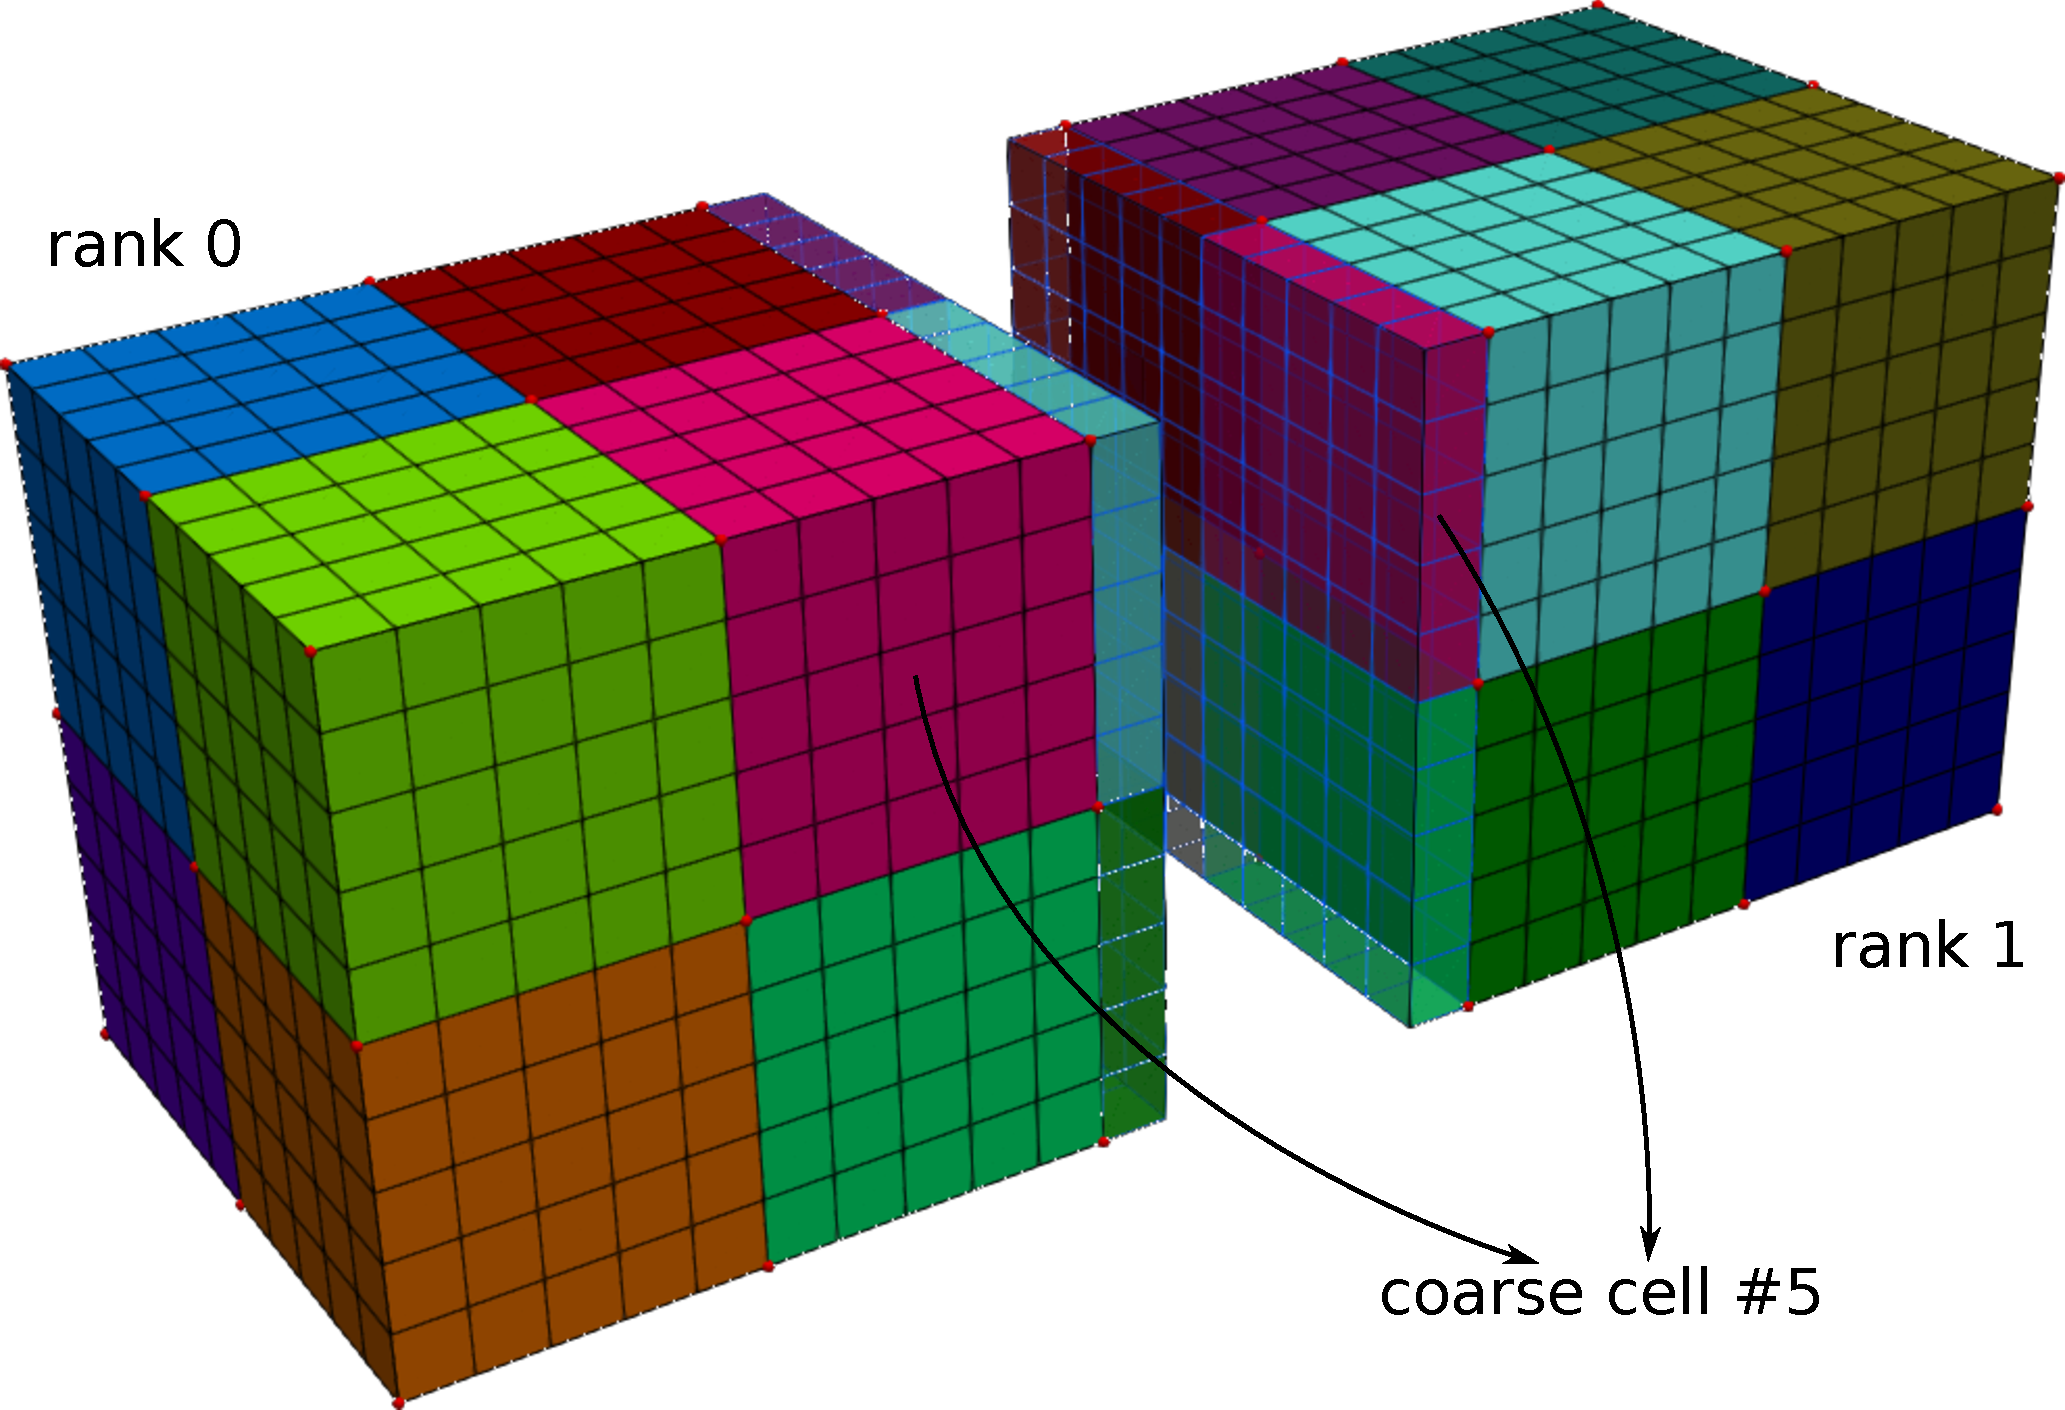
\includegraphics[width=\linewidth]{figs/Cube_parallel_part}}
  \caption{\label{fig:par_decomp_struct}}
\end{subfigure}
\hfill
\begin{subfigure}[t]{0.45\textwidth}
  \centerline{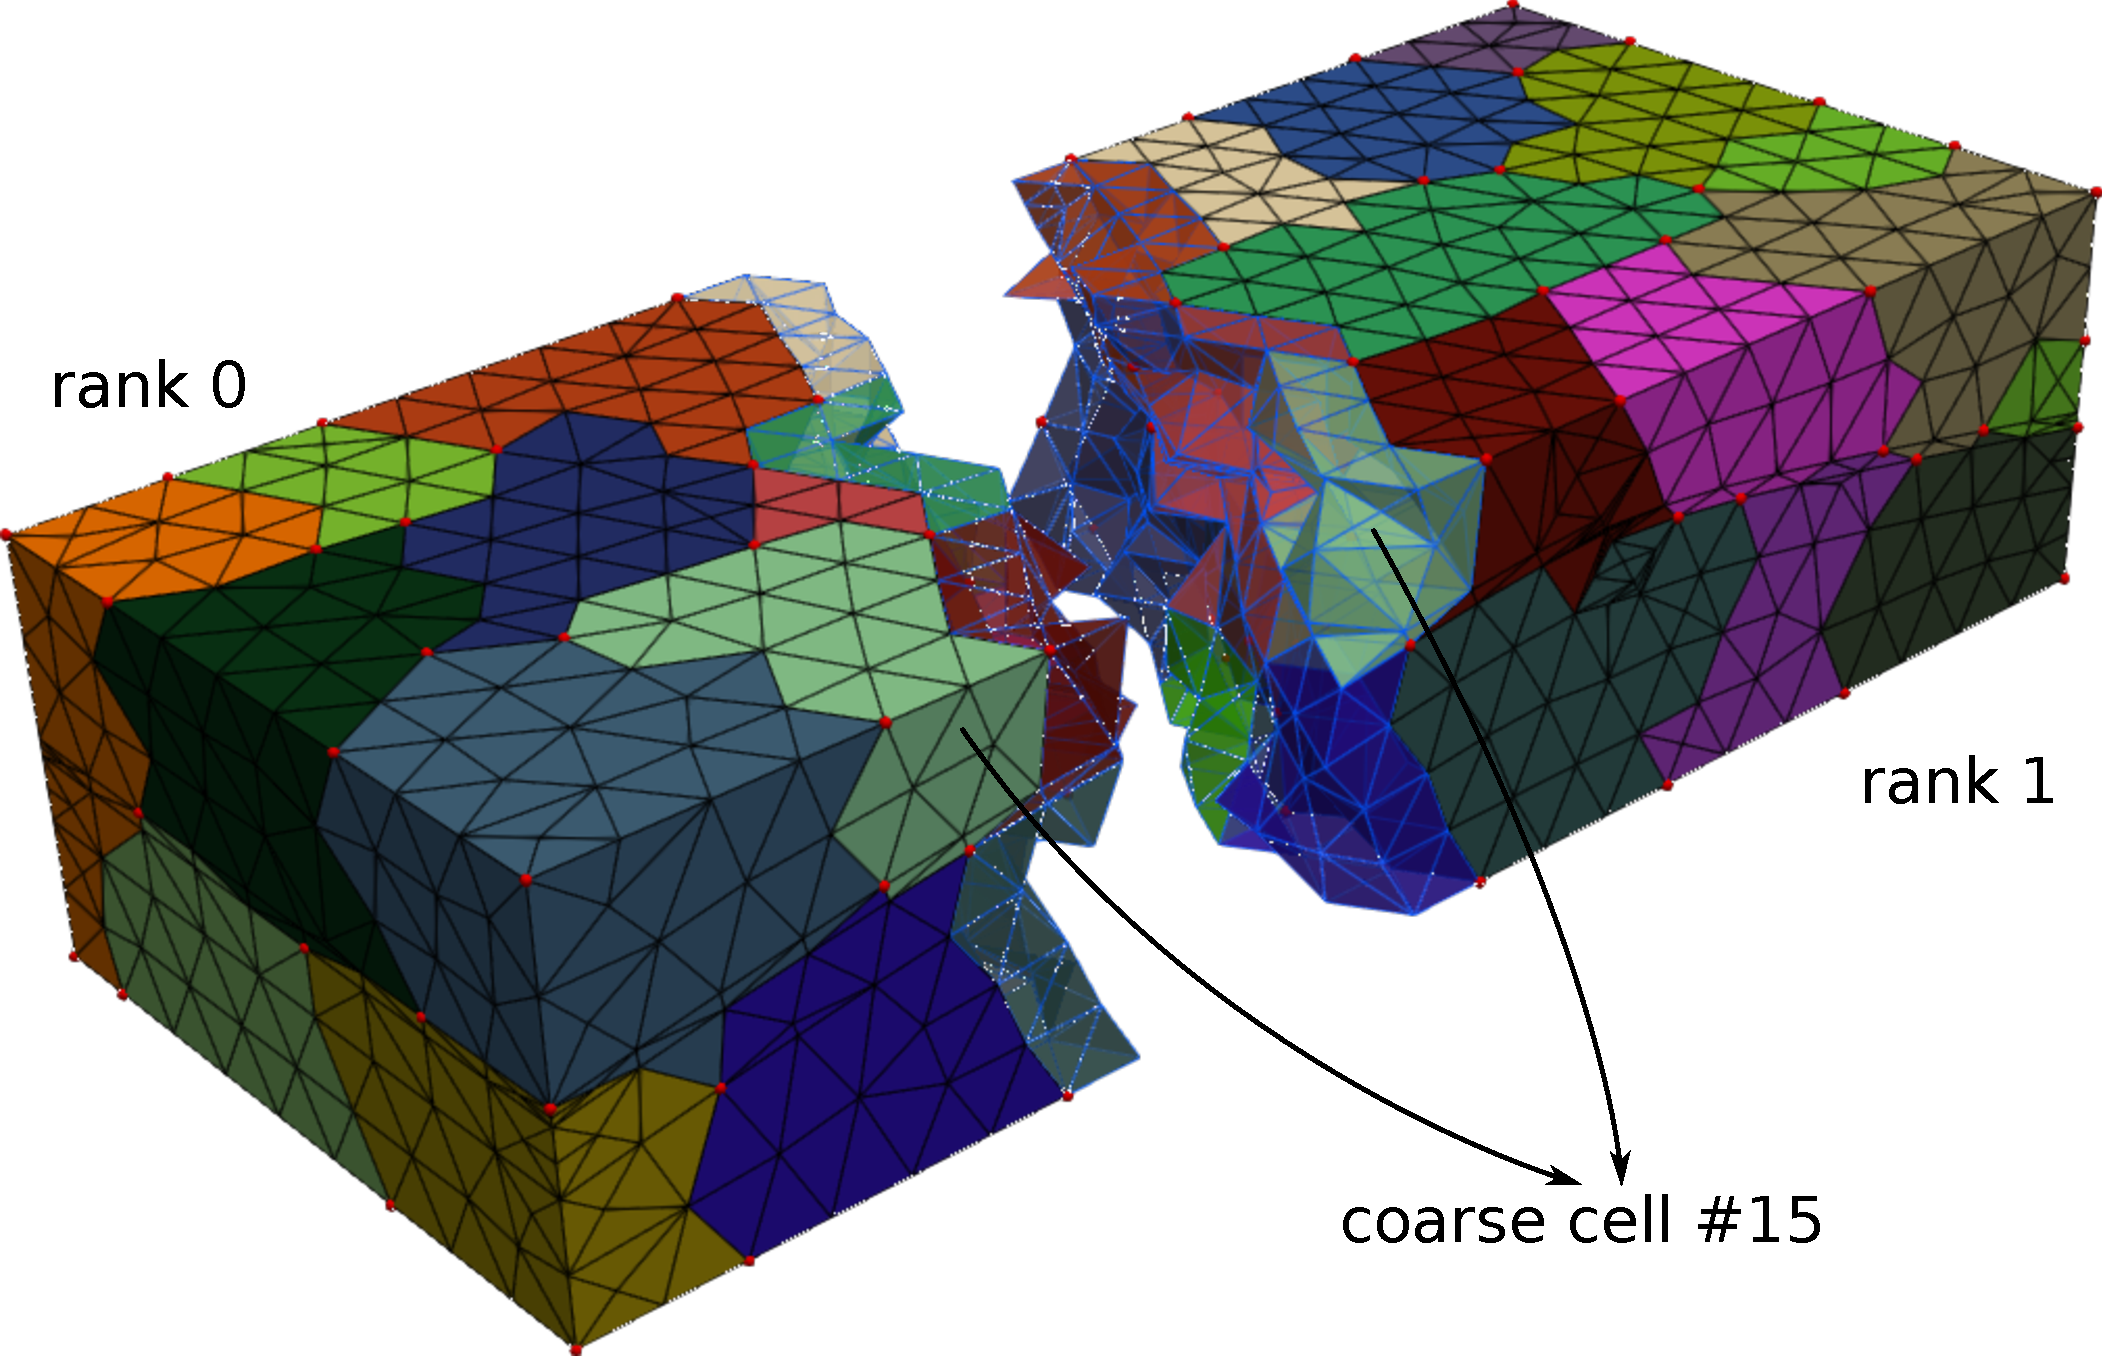
\includegraphics[width=\linewidth]{figs/MazuModel2_parallel_part}}
  \caption{\label{fig:par_decomp_unstruct}}
\end{subfigure}
\caption[Parallel decomposition of multiscale mesh levels]{\label{fig:par_decomp} Parallel decomposition of mesh levels for structured Cartesian (left) and fully unstructured tetrahedral (right) meshes.   Solid colors indicate locally owned cells, while ghosted cells are semi-transparent.   Coarse nodes are shown as \Colorcircle{red}.}
\end{figure}

Compared to the mesh data structure in the main simulation code described in \cref{ch:geosx_framework}, the multiscale mesh is more lightweight and has the following distinctions:
\begin{itemize}
    \item only parts of the domain relevant to the specific physics are represented (for example, if multiscale solver is used for a flow problem defined only in the reservoir zone of a larger physical domain);
    \item faces/edges of the mesh are not stored, and there is no grouping of cells into regions and sub-regions, the numbering of cells is contiguous throughout the domain;
    \item both $\mathcal{G}_E$ and $\mathcal{G}_E^T$ are stored in most general compressed row form using \texttt{ArrayOfSets} data structure;
    \item all locally owned mesh entities are stored together before ghosts, allowing for better data locality when processing the local mesh partition.
\end{itemize}

We note that the mesh data structure described above is only required during the initial construction of level hierarchy and computing the basis function supports for a new problem.   As long as a sequence of linear problems with varying coefficients defined on the same underlying grid is being solved, the interpolation operators can be updated algebraically without use of the mesh information, which can be discarded after initial setup to reduce memory footprint.

\subsubsection{Level Operators}

Each level needs to store prolongation and restriction operators, as well as the coarse-level matrix once it's computed during the setup process.   Given that the framework is targeting fundamentally unstructured problems, level system matrices are stored using very general Compressed Sparse Row (CSR) format, directly using the chosen linear algebra back-end's specific CSR data structures for copy-free interoperability with the library's computational kernels.   We note that while some other sparse matrix representations (most notably ELL) have characteristics favorable for highly vectorized CPU and GPU architectures, CSR is the only format that is widely supported across libraries and has lower memory footprint for highly irregular (i.e. varying number of non-zeros per row) matrices arising from unstructured grid discretizations.

The prolongation operator simultaneously encodes the structure of basis function supports and stores the interpolation weights.   Logically it can be viewed either column-wise, where each column's non-zero values represents the weights attached to a particular coarse-level basis function, or row-wise, with each row containing weights of all coarse basis functions for a single fine-scale degree-of-freedom.   Given that basis functions are designed to have local support (i.e. interpolate a relatively small and compact portion of the domain), the prolongation operator is sparse, and either compressed-column or compressed-row representation is appropriate.   The MsRSB algorithm never manipulates basis functions one-by-one but rather updates the entire operator, and some steps like rescaling the weights \cref{eq:msrsb_rescale} are more optimally implemented as row-wise kernels due to better data locality.   Thus we have chosen to also store the prolongation operator in CSR format.

The restriction operator does not need to be explicitly assembled and stored as long as Galerkin coarse problem definition with $R = P^T$ is used.   An implicit transpose operator is created instead that wraps a handle to $P$ and invokes a transpose sparse matrix-vector multiply (SpMV) kernel when invoked.   For cell-centered degrees-of-freedom the preconditioner also supports the option of using MsFV restriction operator $R = R^{cv} = (P^0)^T$, for which an explicit transpose of the tentative prolongation is computed and stored in CSR format.

Parallel distribution of CSR matrices at each level matches ownership of corresponding fine/coarse support points.   Specifically, each parallel process physically stores a contiguous set of rows corresponding to fine mesh nodes/cells (depending on problem type) owned by that process.   In addition, although CSR columns are not physically distributed, a global column map is created which assigns ownership of a range of columns to the process that owns corresponding coarse mesh nodes/cells.   The underlying data structure may use the map to break locally stored data into ''diagonal'' and ''off-diagonal'' blocks and establish communication patterns for off-processor entries in sparse matrix kernels.

% ===================== SECTION =====================
\section{Computational Kernels}
\label{sec:par_kernels}

The usage of a preconditioner involves a setup/compute phase (executed once prior to start of Krylov iteration) and a solve/apply phase called during the iteration.   Further, MsRSB workflow consists of the following steps:
\begin{enumerate}
\item Setup Phase:
    \begin{enumerate}
        \item Construct the coarse grid.
        \item Select basis supports and build tentative prolongation $P^0$.
        \item Apply restricted smoothing iteration \crefrange{eq:msrsb_update}{eq:msrsb_check} to obtain $P$.
        \item Create a restriction operator $R$.
        \item Setup smoothers if necessary.
        \item Compute coarse-level operator $A^H = RA^hP$.
        \item (Recursively) setup next level.
    \end{enumerate}
\item Solve Phase:
    \begin{enumerate}
        \item Apply pre-smoother $\mathcal{M}_{S,pre}^{-1}$.
        \item Restrict the right-hand side: $\vec{r}^H = R\vec{r}^h$.
        \item (Recursively) perform coarse-grid solve.
        \item Interpolate the error update $\vec{e}^h = P\vec{e}^H$ and update solution $\vec{u}$ and right-hand side $\vec{r}$.
        \item Apply post-smoother $\mathcal{M}_{S,post}^{-1}$.
    \end{enumerate}
\end{enumerate}
In this section we take a more detailed look at practical aspects of parallel implementation for each of the above steps.

\subsection{Coarsening}
\label{subsec:par_kernels_coarsening}

The mesh coarsening procedure is carried out simultaneously on parallel processes and additionally accelerated using multiple threads within each process.   While many steps of the algorithm are implemented using parallel RAJA loop constructs and memory space-aware containers described in \cref{ch:geosx_framework}, we do not consider GPU acceleration for this part of the process, since it is involves primarily manipulation of indices, is heavily memory-bound and is unable to utilize and benefit from abundant compute units available.
 
\subsubsection{Cell Partitioning}
\label{subsubsec:par_kernels_coarsening_cells}

The framework supports a number of ways in which cell agglomerates can be constructed.   As mentioned before, coarse partitions are computed independently on each process only for the locally owned subset of cells, and the chosen method must be compatible with the type and parallel distribution of the mesh.
\begin{itemize}
\item Cartesian partitioning is embarrassingly parallel: each thread is assigned a range of local fine cells, for which a coarse partition index must be computed from its fine index and Cartesian coarsening ratio $C_r = (C_r^x, C_r^y, C_r^z)$.   Since the mesh data structure is designed for unstructured grids and makes no assumptions about a specific numbering of cells, we explicitly store global $ijk$-indices of every cell in a 2D array of size $N_E^h \times n_{sd}$ to facilitate the process.   Semi-coarsening in any given direction (typically $z$) is supported by resetting coarsening ratio in other directions to 1 until every rank is left with a single layer of cells.
\item Unstructured partitioning is largely delegated to an external package: METIS \cite{Karypis1999} or Scotch \cite{Chevalier2008}. The latter is more scalable due to multi-threading support, while the former is serial and unfortunately can often be the bottleneck of coarsening, in addition to some other limitations like the maximum number of partitions supported for large meshes.   Both take cell graph description in CSR format, which is constructed from $\mathcal{G}_E^h$ in parallel: each thread in a process is assigned a range of local cells to compute connectivity for, visits the cell's adjacent nodes through $\mathcal{G}_E$ and then adjacent cells of each visited node though $\mathcal{G}_E^T$, collects, sorts and counts all visited neighbor cells on the thread-private stack space and filters those that match connectivity threshold.   The kernel is executed twice: once to compute the exact number of graph edges (since METIS does not accept a graph description with gaps between rows, the allocated capacity of each row must be equal to its size), and once more to actually populate the list into the target \texttt{CRSMatrix} object which is allocated in between the kernels.   A different procedure is employed if matrix-based weights are to be computed using \cref{eq:graph_matrix_weights}, which involves a thread-parallel loop over matrix rows (it is assumed that the matrix sparsity already provides correct graph connectivity).
\item Semi-structured (2.5D) partitioning is a combination of the above two methods: first, a graph restricted to cells from a single layer is built in parallel and partitioned using the unstructured coarsening procedure, then a parallel loop is used to combine surface and z-partition indices into the final coarse partition number.   Similar to the structured case, we store explicit ''column'' and ''layer'' indices in a 2D array of size $N_E^h \times 2$ at every level.
\end{itemize}
Once all processes have partitioned their owned portions of the domain, a process-parallel exclusive scan is performed to adjust the global numbering of coarse cells, followed by global halo synchronization that exchanges partitioning information of ghost coarse cells.   Thus all processes have a consistent view of the distributed partitioning vector $\vec{z}_E^h$ required for the next step.   Aside from potential bottlenecks in graph partitioning packages, this stage is scalable as it is fully threaded only involves a single collective communication (scan) and neighbor point-to-point exchanges.

\subsubsection{Coarse Node Selection}
\label{subsubsec:par_kernels_coarsening_nodes}

Coarse nodes are selected following the algorithm presented in \cref{subsec:msrsb_coarsening_algorithm} adjusted for parallel processing.   The first step is computing the coarse subdomain adjacency, $\mathcal{G}_S$.   Each thread processes a range of fine nodes, visiting adjacent fine cells through $\mathcal{G}_E^h$ and collecting unique (global) partition indices for those cells from $\vec{z}_E^h$.   In addition, virtual (boundary) subdomains are handled by parallel loops over corresponding node sets.   The results are collected in an \texttt{ArrayOfSets} data structure, which guarantees that values in each sub-set are sorted and unique.   Thus each row is a compact representation the key $K_i$ of node $i$ (the set of adjacent coarse subdomains).   At this point all nodes $i$ that have $|K_i| < 3$ are removed from consideration, significantly reducing processing cost and memory footprint.   We then perform a halo exchange of $\mathcal{G}_S$ sending rows (egde sets) of shared nodes from owning processes to non-owning neighbors, so that nodes located on the outer boundary of halo layer receive their full adjacency information.    This is critical for being able to perform further analysis in a local manner correctly.

In the second step the remaining nodes on each process are sorted according to their keys using lexicographical comparison of sorted sub-arrays representing $K_i$ (which is a weak total ordering).   We use a multi-threaded sort implementation provided by RAJA, which internally employs recursive merge-sort with tasking to achieve good load balancing between threads.   The sorting is heavily memory-bound since keys need to be accessed multiple times, and the amount of exposed parallelism is limited at final levels of the merge tree, but overall this step is quick since a relatively small fraction of nodes is processed.   After that grouping of nodes into features is performed by linearly scanning the sorted nodes, which is optimally done by a single thread but is very fast in practice.

The third step involves building a feature adjacency graph $\mathcal{G}_F$, which is also a memory-bound, trivially-parallel kernel.   Each thread populates connectivity for a subset of features, traversing several adjacency lists, and while the amount of data that needs to be accessed for each feature is large (feature-to-node, node-to-cell, cell-to-node, node-to-feature maps), the end result is a very compact \texttt{ArrayOfSets} data structure since only a ''edge skeleton'' subset of nodes is considered.   Finally, one more thread-parallel loop over features is employed to walk the feature connectivity and check the keys associated with each feature.   One of feature's nodes is marked as a coarse node if its key is not included in any of the neighbors' keys (easy to check with keys being sorted sets).

Each process follows the steps above to process its owned fine-scale nodes and mark coarse nodes.   A halo exchange is used to communicate coarse-node selection status of each node to the non-owning neighbors, and a process-wide parallel exclusive scan is once again needed to establish a consistent global numbering or coarse nodes.   This stage is also scalable with respect to both shared- and distributed-memory computing, since it involves mostly trivially parallel local work and limited communication.

\subsection{Interpolation operators}
\label{subsec:par_kernels_support}

The next phase of setup is building the tentative prolongation operator.   Here we describe how the algorithms proposed in \cref{sec:msrsb_interpolation} are implemented efficiently in a parallel setting.   This involves:
\begin{enumerate}
    \item Computing the supports structure, i.e. the sparsity pattern of $P$
    \item Filling in initial partition of unity (the only near-null space vector we consider)
    \item Computing the global support boundary, i.e. the set of rows of $P$ that must be rescaled.
\end{enumerate}

\subsubsection{Nodal Basis Supports}
\label{subsubsec:par_kernels_support_nodes}

The support of a nodal basis function consists of all fine-scale nodes located strictly within the union of coarse subdomains (including virtual/boundary ones) adjacent to the coarse node associated with the basis function.   This can be realized in one of two ways:
\begin{itemize}
    \item by processing basis functions one by one and collecting a list of fine nodes according to the above definition;
    \item or by processing each fine node and inserting it into support of each adjacent basis function as appropriate.
\end{itemize}
The first approach is more natural to implement, but the second one exposes more fine-grained parallelism and allows for better load balancing across threads.   Moreover, with the row-oriented storage chosen for $P$, the sparsity pattern is more performant to construct in a row-wise manner.   Therefore in our algorithm each thread is assigned a range of fine-scale nodes (rows of $P^0$).   It visits coarse subdomains adjacent to the fine node utilizing the node-subdomain graph $\mathcal{G}_S$ previously described, builds the candidate list of relevant coarse nodes and checks its key $K_i$ against the key $K_j$ of candidate coarse node $j$.   Any node $i$ that belongs to a coarse volume interior ($|K_i| = 1$) is immediately added to the support of all adjacent basis functions.   Otherwise $i$ is included in support of $j$ \textit{iff} $K_i \subseteq K_j$, i.e. $i$ is not adjacent to any subdomain that is not in $j$'s ''area of influence''.   This is a trivially parallel kernel that requires no synchronization, though it must be executed twice: first computing the required capacity of each row, then actually filling the rows of sparsity pattern, allocating memory in between the two.   In a distributed memory setting, each process constructs sparsity for rows corresponding to its owned nodes.   Because the mesh data structure maintains a synchronized halo of both coarse cells and nodes, each process can correctly assign the full set of interpolating basis functions to each fine node without additional communication.

To construct initial partition of unity, we implement a parallel version of nodal clustering algorithm described in \cref{subsec:msrsb_nodal_basis}.   The algorithm maintains a list of nodes that need cluster assignment (the ''expansion front''), initially containing just the list of coarse nodes.   At every iteration, nodes in the list are distributed evenly among worker threads, each node's neighbors are visited and the node is assigned to the cluster that the majority of its neighbors are in.   Additional checks are made to ensure a node is not assigned outside of coarse basis functions' support.   Then, a new list is built by collecting neighbors of the current list that are still not assigned.   We use hardware atomic add instructions (through a portable interface available in RAJA) to coordinate appending new entries to the list from multiple threads in an efficient manner.   The algorithm terminates when the front becomes empty, i.e. all nodes have been assigned, and produces a fine-scale nodal partitioning vector $\vec{z}_N^h \in [1,N_N^H]^{N^h}$.    We then set $P_{ij}^0 = 1 \Leftrightarrow [\vec{z}_N^h]_i = j$.   No parallel communication is required, because two processes with a shared boundary are guaranteed to independently produce equivalent assignments of nodes on the process boundary to the clusters corresponding to coarse nodes located on the same shared boundary.   This is a consequence of the chosen coarsening strategy (matching coarse cells to process subdomain boundaries) and support definitions.

\subsubsection{Cell Basis Supports}
\label{subsubsec:par_kernels_support_cells}

To define support of a cell-centered basis functions, we start by building the nodal clusters as described in \cref{subsubsec:par_kernels_support_nodes}.   We then employ the algorithm described in \cref{subsubsec:par_kernels_support_nodes} to build a coarse subdomain adjacency graph $\mathcal{G}_S^*$, however flipping the roles of cells and nodes: nodal partitions $\vec{z}_N^h$ now define subdomains and fine cells play the role of fine-scale objects whose adjacency is required.   Finally, the support sparsity pattern is built using the same algorithm as in \cref{subsubsec:par_kernels_support_nodes} but with $\mathcal{G}_S^*$ as the input instead of $\mathcal{G}_S$.   The support of a basis function associated with a coarse cell is thus comprised of fine cells that belong exclusively to the union of nodal partitions originating from the coarse cell's nodes.   Here we avoid explicitly computing and post-processing the coarse dual grid and immediately construct ''merged'' supports (as defined in \cref{subsec:msrsb_cell_basis}.   Initial partition of unity is produced simply using existing coarse cell partitions: we assign $P_{ij}^0 = 1 \Leftrightarrow [\vec{z}_E^h]_i = j$.   The construction of cell supports is thus also communication-free.

\subsection{Restricted Smoothing}
\label{subsec:par_kernels_msrsb}

The most computationally intensive part of the setup is the calculation of basis functions via restricted smoothing \crefrange{eq:msrsb_update}{eq:msrsb_check}.   This can be done on the CPU or the GPU if the linear algebra back-end (e.g. \textit{hypre}) is built with GPU support.   The implementation of each step is described below.

\subsubsection{Iteration Matrix}
\label{subsubsec:par_kernels_msrsb_matrix}

The $\ell_1$-Jacobi iteration matrix of \cref{eq:msrsb_update} given by 
\begin{align}
    G = I - \omega D^{-1} \widetilde{A} \label{eq:msrsb_iteration_matrix}
\end{align}
can either be applied implicitly (as a sequence of elementary matrix operations) or built explicitly.   Given that the operations involved need to be applied many times during the course of smoothing iteration, we pre-compute it to minimize both floating point operations and kernel launch overhead.   This involves the following steps:
\begin{enumerate}
    \item Separate component filter removes entries corresponding to coupling blocks from the sparsity pattern according to \cref{eq:blk_stiff_SDC}.   This step is only needed when number of degree-of-freedom components is greater than 1 (e.g. for mechanics problems).   In our implementation unknowns are ordered by collocation point, so the sparsity pattern is compressed afterwards to avoid wasting memory bandwidth.
    \item The M-matrix enforcement kernel applies \crefrange{eq:msrsb_mpfa_filtering_offd}{eq:msrsb_mpfa_filtering} to each row modifying the entries as appropriate, but preserving the sparsity pattern.
    \item Compute $G$ via \cref{eq:msrsb_iteration_matrix}.   Since $G$ has the same sparsity pattern as $\widetilde{A}$, the modification is done in-place.   Left multiplication by $D^{-1}$ amounts to row scaling of $\widetilde{A}$, therefore the entire kernel is also mapped to threads and executed row-wise.
\end{enumerate}
All kernels operate directly in the target memory space (CPU or GPU) and no parallel communication is required.   The execution is memory-bound on both architectures.    A more optimal implementation on the GPU can be achieved by assigning a warp of threads per row instead of a single thread and accessing values in a coalesced manner; however this is more difficult to express in the RAJA programming model and is outside the scope of this work.

\subsubsection{Prolongation Update}
\label{subsubsec:par_kernels_msrsb_update}

The computation of prolongation operator update is the most computationally intensive part of MsRSB setup.   It is implemented in four steps:
\begin{enumerate}
    \item Compute the next candidate $\bar{P}^{n+1}$ via \cref{eq:msrsb_update}.   This is a parallel Sparse Matrix-Matrix (SpMM) multiply operation which extends the support of each basis function in $P^n$ by one layer of points in each direction (according to the stencil of $A^h$).   Parallel communication is required to exchange sets of remote rows that are involved in computation of the local range of result matrix rows; it has the same communication pattern as a standard halo exchange.   A large degree of parallelism is available within each process due to independent computation between rows of the product.   We take advantage of the efficient and carefully optimized SpMM implementations available in the linear algebra back-ends.
    \item Truncate entries of $\hat{P}^{n+1}$ to the sparsity pattern of $P^n$ via \cref{eq:msrsb_restrict}.   This is a local (no communication) memory-bound row-wise operation that primarily involves comparison of multiple column indices and copying values (we keep around a scratch copy of $P^n$ to facilitate this).   We have implemented it as a custom row-wise kernel for each of the backends.   Some libraries don't maintain entries in each CSR row in sorted order; in these cases we first create a sorted ''view'' of each row by computing a corresponding index permutation in auxiliary memory for both source and destination matrices, with the sorting operations carried out by threads in parallel.
    \item Rescaling rows of $\hat{P}^{n+1}$ to unit row sums according to \cref{eq:msrsb_rescale}, which is only performed on a subset of rows of $P$ corresponding to union support boundary.   This is a also fully local and highly parallel kernel.
    \item Convergence check \cref{eq:msrsb_check} which involves computing difference norm between two matrices with identical sparsity patterns.   This operation requires cooperation at the thread and process level to reduce the and broadcast the final norm value.
\end{enumerate}
In a fully optimized implementation steps 1 and 2 could be fused together into a single operation: given a target sparsity pattern, the SpMM kernel might be able to avoid additional work and memory accesses involved in building sparsity pattern of the result and computing entries that are eventually discarded.   Such an implementation is currently not provided by any of the supported linear algebra backends and cannot be developed externally to their respective packages, unlike some of the more straightforward custom kernels (e.g. row rescaling).   We consider this to be an important future optimization of the setup procedure.

In practice, the number of smoothing iterations required to obtain good quality basis functions is on the order of 10--20 on the first application of the preconditioner and 1--5 on subsequent, assuming the matrix changes mildly between nonlinear iterations and simulation time steps.   Note that in general at least one iteration must always be performed in order to assess convergence (unless system the matrix is known to be constant, in which case updating the preconditioner setup can be skipped altogether).   We employ some practical tricks to further reduce computational load without sacrificing robustness, such as only checking convergence every few iterations and adjusting check frequency based on previous convergence history.

\subsection{Coarse Operator}
\label{subsec:par_kernels_coarse}

Computation of coarse-scale operator $A^H = RA^hP$ is another computationally intensive kernel in the setup which involves multiple rounds of neighbor communication.   Unlike the restricted smoothing update however, it only needs to be carried out once per setup, therefore its overall impact on setup cost is fairly mild.   Unlike some recent parallel multiscale methods focusing on Cartesian grids \cite{Manea2016,Manea2019,Manea2021}, we cannot exploit a known structure of $P$ to specialize product computation which must handle general sparse matrices.   Linear algebra libraries that contain a multigrid preconditioner typically also provide specialized matrix triple product routines (optimized for the Galerkin case of $R = P^T$); we take advantage of them whenever possible, falling back on two-step general SpMM in other cases.   In practice, we can avoid recomputing the coarse system if the prolongation operator hasn't changed significantly since the previous setup.   The cumulative number of iterations performed in prolongation smoothing since last computation of $A^H$ is used as a proxy metric for the amount of change accumulated in $P$; it is sufficient to only recompute $A^H$ every 5--10 iterations of restricted smoothing.

\subsection{Application of the Preconditioner}
\label{subsec:par_kernels_apply}

\subsubsection{Smoothers}
\label{subsec:par_kernels_apply_smoothers}

The choice of smoother $\mathcal{M}_S$ has a major impact on robustness and scalability of a multilevel preconditioner, since it is responsible for the bulk of the computational work across all levels of the hierarchy.   The requirements for the smoother thus are:
\begin{itemize}
    \item must be efficient at eliminating high-frequency errors
    \item should have a reasonable setup cost and a scalable application kernel
\end{itemize}
Complex smoothers such as incomplete factorizations (ILU family and its block variants) are often a method of choice for a local stage in two-stage preconditioner (CPR) in reservoir simulation.   They are powerful at dealing with local error, but their setup is expensive and not easily parallelizable.   Simple pointwise relaxation schemes such as Jacobi, Gauss-Seidel, on the other hand, have inexpensive setup and are highly scalable, but suffer from weaker convergence characteristics.   The choice of a proper smoother is often problem-dependent and is a balancing act between the above two requirements that are fundamentally at odds.

Our multilevel framework provides the user with a choice from a large number of smoothers that the selected linear algebra backend exposes.   For practical reasons outlined above, present work only considers scalable methods:
\begin{itemize}
    \item Jacobi is a simple smoother with trivial setup and embarrassingly parallel application kernel, but oftentimes lackluster convergence.   Its main benefit is independence of smoothing properties from the number of processors.
    \item (Symmetric) Gauss-Seidel have much better convergence characteristics and are often default choices in multigrid solvers.    Parallelization approaches of GS include red-black ordering (multi-color in general) or hybrid versions in which full GS is applied to processor-wise diagonal blocks while ''off-processor'' entries are lagged by one sweep similar to block-Jacobi.   Despite a seeming dependence on number of processors, hybrid smoothers have been shown to exhibit good smoothing properties independent of parallelism \cite{Baker2011} and are the default choice in \textit{hypre}' BoomerAMG solver \cite{Henson2002}.
    \item Polynomial smoothers (such as Chebyshev) have the advantage of only requiring matrix-vector (SpMV) operations.   The downside is somewhat expensive (though still scalable) setup stage that must perform iterative eigenvalue estimation.   Their convergence and performance properties are often comparable to those of Gauss-Seidel.
\end{itemize}
Pre- and post-smoothers can be selected independently and either of them can be completely disabled.   The number of smoothing sweeps is another problem dependent tuning parameter that must carefully balance additional work per iteration with improvements in convergence.   In addition, we often replace Jacobi and Gauss-Seidel with their $\ell_1$ versions which attempt to guarantee a convergent smoother by using a modified diagonal \cite{Baker2011}.

\subsubsection{Grid Transfer}
\label{subsec:par_kernels_apply_transfer}

Residual restriction, interpolation of coarse-grid error correction and residual update after smoothing are the remaining operations of the solution phase.   All of them are straightforward SpMV kernels (or transpose-SpMV in case of restriction) that are known to be relatively scalable on modern architectures and have highly optimized implementations in linear algebra libraries (e.g. overlapping computation and communication is commonly done).   Overall they take a relatively minor portion of execution time.

% ===================== SECTION =====================
\section{Performance Characteristics}
\label{sec:par_performance}

Estimating theoretical computational complexity of the algorithm in an unstructured grid setting is complicated since connectivity graphs, stencils, coarsening rules, etc. do not necessarily possess regularity that can be exploited for analysis (cf. \cite{Manea2016}).   Moreover, real performance of the method is highly dependent on implementation and hardware architecture details like the relative cost of various memory access patterns.    Therefore we only attempt to sketch out a very approximate estimate of the number of floating point operations (or \textit{flops}) to expose the different factors and parameter choices that affect the cost and show that the cost depends linearly on the problem size.   We make a large number of simplifying and homogenization assumptions about mesh topology, although we don't necessarily assume any specific grid structure.   For simplicity, we limit the discussion to problems with nodal degrees-of-freedom, noting that analysis is similar for cell-centered problems with appropriate adjustments for the averaging constants involved.

\subsection{Notation and Assumptions}
\label{subsec:par_performance_notation}

We consider a multilevel MsRSB scheme with $M$ total levels and use $k$ to denote the grid level, with $k=0$ being the original fine-scale problem.   Let $N_k$ be the number nodes (unknown collocation points) at level $k$.   Moreover, let $C_r = N_k/N_{k+1}$ be the average coarsening ratio set to be constant at every level, where we additionally assume that the ratio is the same for cells and degrees-of-freedom (which is only approximately true for Cartesian grids).   From the above definitions,
\begin{align}
    N_k = \frac{N_0}{(C_r)^k}
\end{align}
and we can introduce, similar to the its use in multigrid literature, the \textit{grid complexity} factor
\begin{align}
    C_g = \frac{1}{N_0}\sum\limits_{k=0}^{M-1} N_k = \frac{1}{N_0}\sum\limits_{k=0}^{M-1}\frac{N_0}{(C_r)^k} = \sum\limits_{k=0}^{M-1}\frac{1}{(C_r)^k} \label{eq:complexity_grid}
\end{align}
Note that $1 \leq C_g \leq 2$ and that $C_g$ decreases as $C_r$ is increased; \cref{eq:complexity_grid} does not account for the change in number of levels $M$ as a function of $C_r$ for fixed problem size, but these observations would still hold.   We also denote $n_d$ to be the number of degrees-of-freedom per point (e.g. 1 for flow and 3 for mechanics), and let $N = n_d N_0$ the total fine-scale problem size.   We introduce additional mesh averaging constants:
\begin{itemize}
    \item $C_s$ is the average stencil size of the problem, i.e. the average number of non-zeros per row of $A^h$.
    \item $C_{en}$ is the average number of coarse elements per coarse node.
    \item $C_{ne}$ is the average number of coarse nodes per coarse element.
\end{itemize}
These values are assumed to remains the same at every grid level, although this only strictly holds true for Cartesian grids and structured coarsening.   In particular, as explained in \cref{sec:msrsb_interpolation}, basis function supports are designed so as to avoid stencil size growth.   The other two ''topological'' factors are empirically observed to remain approximately constant.

In the following, we use the symbol $\mathcal{C}$ to denote computational complexity of various setup stages, or more specifically, the number of floating point multiplications involved (the number of additions is of the same order of magnitude).   Cost of the solution stage is largely dominated by application of smoothers and is not considered here.

\subsection{Iteration matrix}

Computing the iteration matrix $G$ via \cref{eq:msrsb_iteration_matrix} involves only summation of entries of $A$ in each row and later scaling them by inverse diagonal.   The total flop count is thus proportional to number of non-zeros of $\widetilde{A}$ across all levels, which, after separate component filtering, is
\begin{align}
    \mathcal{C}_G = \sum\limits_{k=0}^{M-1} (n_d \times C_s \times N_k) = n_d \times C_s \times \sum\limits_{k=0}^{M-1} \frac{N_0}{(C_r)^k} = N \times C_s \times C_g = O(N) \label{eq:complexity_iter_mat}
\end{align}

\subsection{Prolongation Operator}

Next, we estimate the number of non-zero entries in the prolongation operators across all levels, which is also the flop count of applying prolongation to a coarse-scale vector (or, equivalently, prolongation to a fine-scale vector).   Assume for the moment that we have a single unknown per point, $n_d = 1$.   Then prolongation $P^k$ at level $k$ has $N_{k+1}$ columns corresponding to coarse basis functions, each of which has support inside adjacent dual coarse volumes.   There are $C_{en}$ of these volumes, each with approximately $C_r$ points (we neglect outer boundary of the union of dual volumes that is not part of support, but double-count the overlapping points shared by dual volumes in support).   If $n_d > 1$ (e.g. mechanics), it simply multiplies the number of non-zeros, because an interpolation operator based on separate component approximation matrices $\widetilde{A}$ is decoupled (each ''element'' is a diagonal block of size $n_d \times n_d$).   Then,
\begin{align}
    \mathcal{C}_{P^k} = \Nnz(P^k) \approx n_d \times C_{en} \times C_r \times N_{k+1} = n_d \times C_{en} \times C_r \times \frac{N_0}{(C_r)^{k+1}} = C_{en} \times \frac{N}{(C_r)^k} \label{eq:complexity_prolongation}
\end{align}
Finally the sum across all levels is
\begin{align}
    \mathcal{C}_{P} = \sum\limits_{k=0}^{M-1} \mathcal{C}_{P^k} = C_{en} \times N \sum\limits_{k=0}^{M-1}\frac{1}{(C_r)^k} = N \times C_{en} \times C_G = O(N) \label{eq:complexity_prolongation_all}
\end{align}

\subsection{Restricted Smoothing}

Denote $N_I$ the number of smoothing iterations to be applied (we assume it is prescribed to be the same for all levels, even though levels might take a different number of iterations to converge).   Each smoothing iteration includes the steps below.

\paragraph{Prolongation update}
Computation of next prolongation candidate $\widetilde{P}^{n+1}$ via SpMM \cref{eq:msrsb_update} has the effect of applying the stencil of $\widetilde{A}$ to every point in support of every basis function or, equivalently, every nonzero value in $P^n$.   For $n_d > 1$, row of $G$ and columns of $P^n$ corresponding to different unknown components have no overlap due to unknown decoupling, so they do not contribute to flop count.   Therefore, the total computational cost of the updates is
\begin{align}
    \mathcal{C}_{U} = \sum\limits_{k=0}^{M-1} C_s \times \mathcal{C}_{P^k} = C_s \times \mathcal{C}_P = N \times C_{en} \times C_g \times C_s = O(N) \label{eq:complexity_update}
\end{align}

\paragraph{Truncation}
Restricting the candidate prolongation to prescribed support amounts to comparing indices and copying values, and does not introduce any floating-point operations.

\paragraph{Rescaling}
Rescaling step \cref{eq:msrsb_rescale} is only performed on rows of $P$ corresponding to degrees-of-freedom belonging to the union support boundary.   A very rough estimate of the number of points on the boundary can be obtained as follows: for a coarse dual subdomain, the number of points on its boundary is approximately proportional to its surface area; if coarsening ratio $C_r$ is a measure of ''volume'' of a coarse subdomain in terms of number of points, ''surface area'' measure can be approximated as $C_r^{\frac{2}{3}}$; with all coarse cells combined, points on each shared interface are counted twice, on each shared edge 3 or more times and so on, so a conservative (overestimating) factor of $1/2$ can be used.   The number of non-zero values in each rescaled row of $P$ is the number of coarse points adjacent to the coarse cell interface the fine point is on, which is difficult to estimate analytically; in a 3D Cartesian grid this number is 4 (faces) or 2 (edges), while in some unstructured tetrahedral meshes with METIS coarsening we tested it varies from 2 to 10, however the average remains close to 4 regardless of choice of $C_r$; hence we use 4 as an approximation.   Putting it together, the flop count of rescaling is estimated as
\begin{align}
    \mathcal{C}_{R} = \sum\limits_{k=0}^{M-1}\frac{1}{2}(C_r)^{\frac{2}{3}} \times n_d \times N_{k+1} \times 4 = 2 n_d \times (C_r)^{\frac{2}{3}} \times \sum\limits_{k=0}^{M-1}\frac{N_0}{(C_r)^{k+1}} = N \times \frac{2C_G}{\sqrt[3]{C_r}} = O(N) \label{eq:complexity_rescale}
\end{align}

\paragraph{Convergence check}
The check involves computing maximum absolute difference between elements of two sparse matrices and does not involve floating point multiplications.

\subsection{Galerkin Product}

Computation of coarse-scale system via $A^H = RA^hP$ consists of two steps.   Computing $A^h P$ is equivalent to the prolongation update in restricted smoothing, with the difference that $A^h$ is the full (non-filtered) fine-scale matrix, and thus requires $n_d$ times more flops to account for coupling between unknown components.   Computing the second SpMM product $R(A^hP)$ takes a multiplication for each pair of coarse basis functions that interpolate a given fine degree-of-freedom (as noted in \cref{sec:msrsb_interpolation}, no new connections are introduced at the coarse level).   The number of such pairs on level $k$ can be conservatively estimated to be $N_k \times C_{ne}^2$, assuming every fine node is interpolated from $C_{ne}$ coarse nodes adjacent to the corresponding coarse element (nodes on shared interfaces are actually interpolated from fewer coarse nodes).   The coupling between unknown components introduces an additional factor of $n_d^2$.   Altogether, the computational cost is estimated as
\begin{align}
    \mathcal{C}_{RAP} = N \times C_{en} \times C_g \times C_s \times n_d + \sum\limits_{k=0}^{M-1} N_k C_{ne}^2 n_d^2 = N \times n_d \times C_g \times \left(C_{en} C_s + C_{ne}^2\right) = O(N)
\end{align}

\subsection{Coarse Solver}
Assuming $LU$ factorization with pivoting and fill-minimizing reordering is used as the coarsest level solver, the cost of computing depends on number of unknowns at the coarsest level and bandwidth of the reordered matrix.   The latter is difficult to estimate for arbitrary grids, however we note that since our coarsening algorithms are stencil-size preserving, matrix bandwidth is also expected to remain bounded.   As for number of unknowns, the upper bound for it is typically chosen apriori to be small enough for the coarse solver not to become a bottleneck, and the number of levels is selected until the desired bound is satisfied.   Thus the cost of coarse solver setup is independent of fine-scale problem size, which is a departure from two-level multiscale methods (cf. \cite{Manea2016}).

% ===================== SECTION =====================
\section{Numerical Results}
\label{sec:par_results}

In this section we present several numerical examples that investigate robustness and parallel scalability of the multiscale preconditioner implemented in GEOSX on multi-core and multi-node architectures.   We also look at relative costs of different kernels of the setup stage in an optimized implementation.   Some comparisons with a state-of-the art classical multigrid solver are provided to validate the observed performance of the method.

\subsection{Test Cases Setup}

\subsubsection{Computational Platform}

\paragraph{Hardware specifications} All tests are run on Stanford Computation Earth and Environmental Sciences (CEES) Mazama HPC cluster, consisting of up to 150 compute nodes connected with a Mellanox Infiniband FDR (56 Gb/s) interconnect.   Each node features 64 GB of DDR4 RAM and dual-socket Intel\textsuperscript{\tiny\textregistered} Xeon\textsuperscript{\tiny\textregistered} E5-2670 v3 (Haswell microarchitecture) CPU with 30 MB of shared L3 cache and 12 cores per socket operating at \qty{2.3}{\GHz}, each with 256 KB L2 cache and 32 KB L1 data and instruction caches.   The cores support superscalar execution and AVX2 SIMD instruction set.

\paragraph{Software configuration}
The nodes are running a 64-bit CentOS 7.9 with Linux Kernel 3.10.   GEOSX is compiled with GNU C++ Compiler 8.3.0 with \texttt{-O3} optimization level and OpenMP support and linked with Open MPI 3.1.4, METIS 5.1.0, SuperLU\_DIST 6.2.0 and SuiteSparse 5.10.1.   We use \textit{hypre} 2.24.0 \cite{hypre} as the linear algebra backend and BoomerAMG \cite{Henson2002} as the reference classical multigrid preconditioner.    BoomerAMG is configured to employ a single V-cycle with one sweep of the same pre- and post-smoother used in our multiscale solver ($\ell_1$ symmetric Gauss-Seidel), combined with HMIS coarsening, ''extended+i'' interpolation and a direct solver at the coarsest level (set to have a maximum size of 9).   For mechanics problem, we additionally set the connection strength threshold to a recommended value of 0.8 (default is 0.25 for scalar equations) and instruct the solver to use systems variant with 3 functions (PDEs) per point.

\subsubsection{Common Settings}

Similar to the examples presented in \cref{sec:msrsb_examples}, we define three types of problems on each model (geomechanics, single-phase flow and coupled poromechanics) using finite element discretization for mechanics and TPFA finite volume for flow.   Solid skeleton is assumed to be isotropic linear elastic with incompressible grains, while a bulk rock compressibility coefficient of $c_r = \qty{1e-9}{\Pa^{-1}}$ is used in the flow problem.   Fluid is also assumed to have constant compressibility of $c_f = \qty{5e-10}{Pa^{-1}}$, viscosity $\mu = \qty{1e-3}{Pa.s}$ and density $\rho_f = \qty{1000}{kg/m^3}$, while gravity is neglected.   The resulting flow and poromechanical problems are time-dependent and mildly nonlinear, while geomechanical problem is linear and quasi steady-state (with time-dependent boundary conditions).

In all cases, we run each problem for 10 time steps and average performance metrics (iterations and timings) over the steps.   In the context of time-dependent problems an expensive part of multiscale setup (coarsening and construction of the grid hierarchy, as well as initial convergence of the basis functions) is amortized across many time steps, while a small number of additional smoothing iterations are sufficient to evolve the grid transfer operators as system matrix changes in the course of the simulation.   In addition, in order to optimize the setup cost, we use a relaxed tolerance of $\varepsilon_{\text{sm}} = \num{1e-1}$ as convergence criteria for basis functions and limit the number of smoothing iterations to 20.   Since the problems considered here do not produce symmetric matrices (in case of mechanics, due to non-symmetric treatment of Dirichlet boundary conditions in GEOSX), we use right-preconditioned GMRES as the iterative solver with a convergence tolerance of $\varepsilon_r = \num{1e-8}$.

\subsubsection{Test Case 1}

The first test represents a \qtyproduct{1x1x0.1}{\km} domain that is discretized with a Cartesian grid using an equal number of cells in $x$, $y$ and $z$ directions, which creates an anisotropy factor of 10 between horizontal and vertical cell dimensions.   This geometric anisotropy is typical in subsurface modeling where grids are highly resolved in the vertical direction, and must be handled robustly by the solver.   Grid resolution levels and corresponding problem sizes are summarized in \cref{tab:cart_dims}.   The time step size for all three problems is chosen to be $\Delta t = \qty{1e5}{s}$.

\paragraph{Flow}
We employ sequential Gaussian simulation to generate a high-resolution geostatistical horizontal permeability field realization spanning over 4 orders of magnitude and map it onto each computational grid using nearest point interpolation. The result for a \numproduct{70x70x70} grid is shown shown in \cref{fig:cart_perm}.   Vertical permeability $k_z$ is obtained by multiplying $k_x$ by an material anisotropy factor set to a default value of \num{1e-2}.   The total numerical anisotropy for this problem is thus \num{1e-1}.    Reference porosity is constant and equal to 0.2 everywhere.   Domain boundaries are no-flow and two wells in opposing corners of the domain completed in layers 2 and 4 (out of 5 equally sized horizontal layers)  impose a varying in time pressure gradient, with producing well set to constant pressure of \qty{10}{\MPa} and injector operating at a constant mass rate of \qty{10}{kg/s}.

\paragraph{Geomechanics}
A heterogeneous Young's modulus distribution is prescribed using the log-permeability correlation \cref{eq:young_perm_correlation} with $\bar{E} = \qty{5}{\GPa}$ and $E_{\max} = 1.5 \bar{E} = \qty{7.5}{\GPa}$, shown in \cref{fig:cart_young}.   Boundary conditions consist of the usual constrained normal displacement on the bottom and side surfaces; in addition, normal traction of \qty{10}{\MPa} (with linear ramp-up as a function of time) is prescribed on the top surface, resulting in a displacement profile that is mostly vertical with small lateral deformation due to material heterogeneity, as shown in \cref{fig:cart_mech_sketch}.

\paragraph{Poromechanics}
The setup consists of a combination of flow and mechanics problems, ignoring the prescribed compression and using only the pressure gradient from wells to drive both flow and solid deformation.

\paragraph{}
Structured coarsening is used in the multiscale solver to generate a hierarchy of Cartesian coarse grids, with a default coarsening ratio of $C_r = \numproduct{5x5x5}$.   In addition, to overcome challenges associated with anisotropy, we employ semi-coarsening in the $z$ direction until each process has no more than a single coarse cell layer.   In distributed memory experiments, parallel partitioning of the domain is also structured, with processes arranged in a Cartesian grid of as even shape as possible.

\begin{figure} [htbp]
    \begin{subfigure}{0.48\textwidth}
        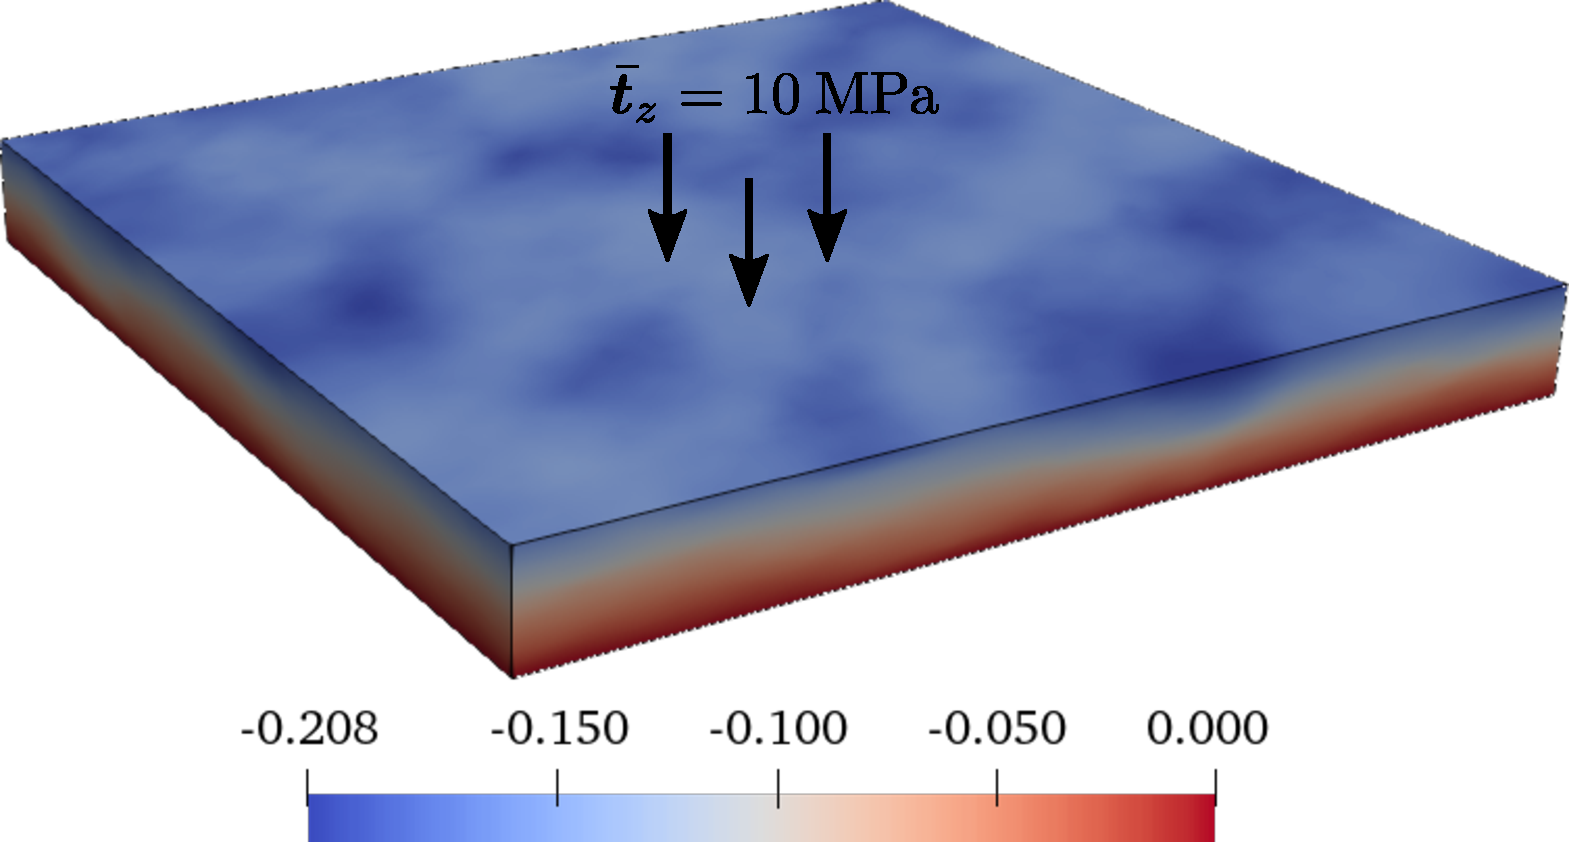
\includegraphics[width=0.9\linewidth]{figs/Cart/mech_sketch_v2}
	    \caption{Mechanics problem and solution, $u_z$ [m]}
        \label{fig:cart_mech_sketch}
    \end{subfigure}
    \hfill
    \begin{subfigure}{0.48\textwidth}
        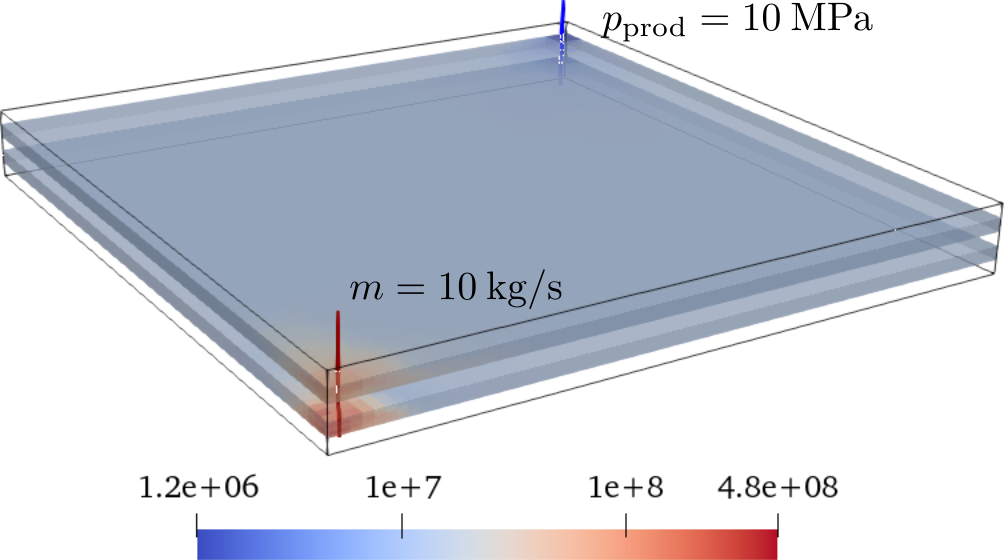
\includegraphics[width=0.9\linewidth]{figs/Cart/flow_sketch}
	    \caption{Flow problem and solution, $p$ [Pa]}
        \label{fig:cart_flow_sketch}
    \end{subfigure}
    \par\bigskip
    \begin{subfigure}{0.48\textwidth}
        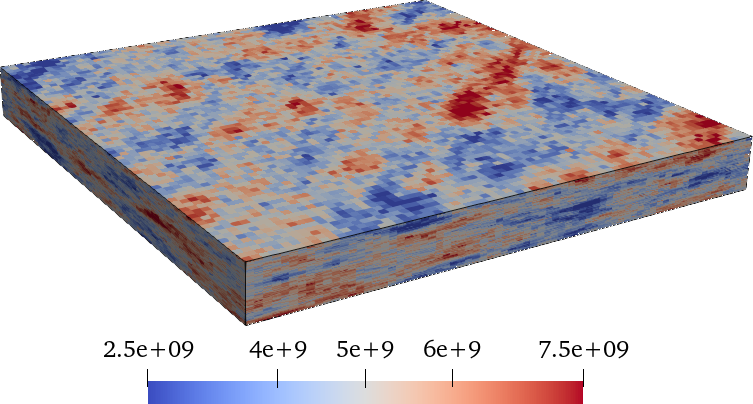
\includegraphics[width=0.9\linewidth]{figs/Cart/young}
	    \caption{Young's modulus, $E$ [Pa]}
        \label{fig:cart_young}
    \end{subfigure}
    \hfill
    \begin{subfigure}{0.48\textwidth}
        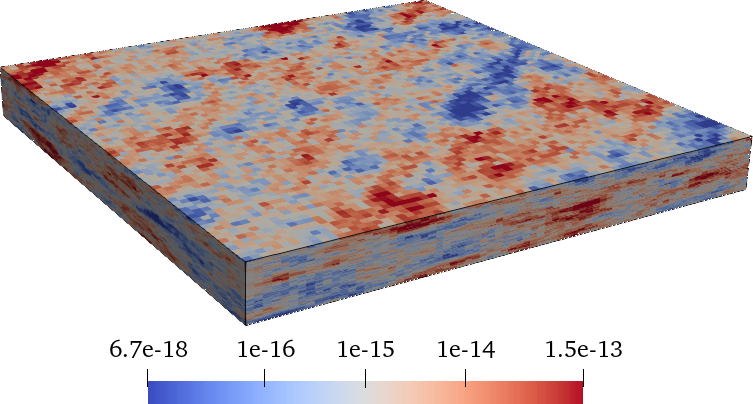
\includegraphics[width=0.9\linewidth]{figs/Cart/perm}
	    \caption{Permeability $k_x$ [\unit{m^2}]}
        \label{fig:cart_perm}
    \end{subfigure}
    \caption[3D Cartesian test case]{3D Cartesian test case: mechanics (a) and flow (b) problem setup and solution at $t = \qty{1e6}{s}$, material properties (c,d).}
    \label{fig:cart_setup}
\end{figure}

\begin{table}
    \centering
    \caption[3D Cartesian problem sizes]{3D Cartesian test case: grid resolution levels and corresponding problem sizes}
    \label{tab:cart_dims}
    \begin{tabular}{crrrr}
      \hline\noalign{\smallskip}
      \multirow{2}{*}{$\ell$} & & \multicolumn{3}{c}{degrees-of-freedom} \\
      \noalign{\smallskip}\cline{3-5}\noalign{\smallskip}
      & & flow & mechanics & coupled \\
      \hline\noalign{\smallskip}
           35x35x35 & &     42,875 &    139,968 &    182,843 \\
           44x44x44 & &     85,184 &    273,375 &    358,559 \\
           56x56x56 & &    175,616 &    555,579 &    731,195 \\
           70x70x70 & &    343,000 &  1,073,733 &  1,416,733 \\
           88x88x88 & &    681,472 &  2,114,907 &  2,796,379 \\
        100x100x100 & &  1,000,000 &  3,090,903 &  4,090,903 \\
        111x111x111 & &  1,367,631 &  4,214,784 &  5,582,415 \\
        140x140x140 & &  2,744,000 &  8,409,663 & 11,153,663 \\
        176x176x176 & &  5,451,776 & 16,635,699 & 22,087,475 \\
        200x200x200 & &  8,000,000 & 24,361,803 & 32,361,803 \\
        222x222x222 & & 10,941,048 & 33,268,701 & 44,209,749 \\
        280x280x280 & & 21,952,000 & 66,564,123 & 88,516,123 \\
      \hline\noalign{\smallskip}
    \end{tabular}
\end{table}

\subsubsection{Test Case 2}

The second example is built using a sequence of three-dimensional unstructured meshes based on a layered reservoir model described in \cref{subsec:msrsb_examples_setup}.

\subsection{Scaling and Parallel Efficiency Studies}

\subsection{Optimal Parameters Choices}

\subsection{Comparison with AMG}

% ===================== SECTION =====================
\section{Summary}
\label{sec:par_summary}